\documentclass[10pt]{exam}
\usepackage[hon]{template-for-exam}
\usepackage{endnotes,graphicx}
\usepackage{tikz,graphicx,enumitem,multicol,float,my-tikz-clipart,silence,cclicenses}
\graphicspath{{./figures/}}
\WarningFilter{latex}{Label `part}
\WarningFilter{latex}{There were multiply-defined labels}

\footer{}{\thepage}{\sc \myclass}


%\def\answer#1{\footnotetext{#1}}
%\def\myquestion{\item\stepcounter{footnote}}

\def\enoteheading{}
\def\answer#1{\endnotetext{#1}}
\def\theanswers{\theendnotes}
\def\myquestion{\item\stepcounter{endnote}}

\newenvironment{myquestions}{
  \begin{multicols}{2}\begin{enumerate}[resume]
}{
  \end{enumerate}\end{multicols}
}
\makeatletter
\patchcmd{\enit@setresumekeys}{\def}{\gdef}{}{}
\patchcmd{\enit@setresumekeys}{\def}{\gdef}{}{}
\makeatother

\newcommand{\myheading}[1]{\uplevel{\section*{#1}}
}
\newcommand{\mysubheading}[1]{\uplevel{\subsection*{#1}}
}

%uncomment if running Pandoc
% \renewcommand{\myheading}[1]{{\section*{#1}}}
% \renewcommand{\mysubheading}[1]{\subsection*{#1}}





\def\mytitle{Chapter 16B Homework (Waves)}
\title{\mytitle}
\date{\today}

\def\mymaketitle{
  \begin{flushleft}
    {\LARGE \textbf \mytitle \par}
  \end{flushleft}
}

\newcommand{\bs}[2]{\textbf{#1} (\sc #2 Points)}


\newcommand{\GFig}[2]{  
  \begin{figure}[H]
    \centering
    \includegraphics[width=#2]{11_#1_Figure.jpg}
    \caption{Giancolli Figure 11-#1.}
    \label{11-#1}
  \end{figure}
}


\begin{document}
\maketitle
% \begin{center}
%   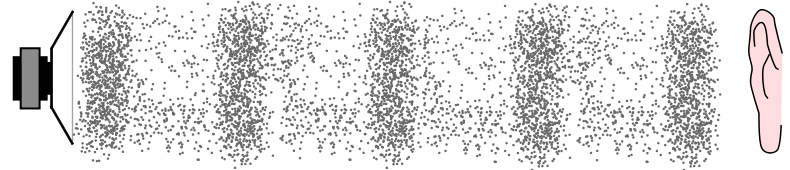
\includegraphics[width=10cm]{sound-wave.png}
% \end{center}

\noindent
We're trying a new format for HW for this mini-unit.  All of your work should go on this packet.  There will be no stamps given.  Instead, you will turn this packet in on test day.  Selected answers are provided on the back page of this packet. \textbf{Your test will be on Wed, Apr 15 (Pd 2) / Thu, Apr 16 (Pd 3, 5)}.  

\vspace{1em}
\hrule
\subsection*{Equations}

\begin{align*}
  v &= f \lambda &
  f_n &= \frac{nv}{2L} = nf_1 &
  f_{BEAT} &= \left|f_1-f_2\right| %s\\
  %f' &= f\left( \frac{v_{snd}\pm v_{obs}}{v_{snd}\mp v_{src}} \right) &&&
  %v_{snd} &= 343~\text{m/s at 20$^\circ$C}
\end{align*}
\hrule

\vspace{1em}

\noindent
Questions and figures are from OpenStax \emph{College Physics} Giancolli \emph{Physics: Principles with Applications}, 7th ed, (Chapter 11) unless otherwise noted.


\section*{Waves Basics Concepts}


\begin{enumerate}[resume]

\myquestion (Original Question) 
  What is the difference between transverse and longitudinal waves? \vs

\myquestion (Giancoli Ch 12, CQ11, modified) Explain how the existence of music is evidence that the speed of sound in air does not depend on frequency.
\vs


\myquestion (Giancoli CQ15) A wave transports which of the following? \answer{A}

\begin{oneparchoices}
  \choice energy but not matter
  \choice matter but not energy
  \choice both energy and matter 
\end{oneparchoices}

\myquestion (Giancoli CQ12)  \answer{straight up $\uparrow$}
Consider a wave on a string moving to the right as shown in Figure~\ref{11-50}.  What is the direction of the velocity of a particle of string at point B?  How do you know
\begin{multicols}{2}
\GFig{50}{7cm}
\end{multicols}



\end{enumerate}


\pagebreak

\section*{Waves Basics Problems}

\begin{multicols}{2}\begin{enumerate}[resume]

\myquestion (Giancoli P35) \answer{2.3 m/s}
  A fisherman notices that wave crests pass the bow of his anchored boat every 3.0 s. He measures the distance between two crests to be 7.0 m. How fast are the waves traveling?
  
\myquestion (Giancoli P36) \answer{1.22 m}
  A sound wave in air has a frequency of 282 Hz and travels with a speed of 343 m/s. How far apart are the wave crests (compressions)?
  
\myquestion (Giancoli P38) \answer{190 m to 545 m; 2.8 m to 3.4 m} 
  AM radio signals have frequencies between 550 kHz (kilohertz) and 1600 kHz and travel with a speed of \SI{3.0e8}{m/s}. What are the wavelengths of these signals? On FM the frequencies range from 88 Mhz (megahertz) to 108 MHz  and travel at the same speed. What are their wavelengths? (\emph{Hint}: $\SI{1}{kHz} = \SI{e3}{Hz}$ and $\SI{1}{MHz} = \SI{e6}{Hz}$)

\myquestion (Original Problem) \answer{(a) 341.3~m/s; (b) 0.74~m; (c) \SI{2.19e-3}{s}}
  A hiker shouts toward a vertical cliff 826~m away.  The echo is heard 4.84~s later. (a) What is the speed of this sound wave in the air? What is the (b) wavelength and (c) period of this wave if its frequency is 456 Hz?

\end{enumerate}\end{multicols}

\pagebreak


\pagebreak

\section*{Standing Waves \& Resonance Problems}

\begin{myquestions}
\myquestion (Giancoli P49) \answer{440 Hz; 880 Hz; 132 Hz; 1760 Hz}
If a violin string vibrates at 440~Hz as its fundamental frequency, what are the frequencies of the first four harmonics?

\myquestion (Giancoli P51, modified)  \answer{(a) 60 Hz, 120 Hz, 180 Hz; (b) 1.50~m}
A particular string resonates in four loops at a frequency of 240~Hz. (a) Give at least three other frequencies at which it will resonate. If the speed of sound on the string is 108~m/s, how long is the spring?
\vs

\myquestion (Giancoli P52)  \answer{0.102 m}
The speed of waves on a string is 97 m/s. If the frequency of standing waves is 475~Hz, how far apart are two adjacent nodes?

\myquestion (Original Problem)  \answer{0.85 m}
How long should a string be in order to produce a standing wave with nine loops using a string oscillator of 180~Hz if the tension is adjusted so that the speed of the wave is 34~m/s?

\myquestion (Original Problem) \answer{(a) 7$^\text{th}$; (b) 0.4 m; (c) 84 m/s; (d) 30 Hz}
Consider a string of length 1.4~m fixed at both ends. When the string vibrates at a frequency of 210 Hz, the standing wave shown below in Figure~\ref{standing} is shown.  (a) Which harmonic is this? (b) What is the wavelength? (c) Determine the velocity of these waves along the string. (d) Determine the fundamental frequency of this string.

  \begin{figure}[H]
    \centering
    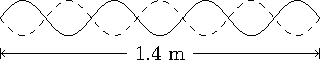
\includegraphics[width=7cm]{standingwave.pdf }
    \caption{(Original Figure) A standing wave on a 1.4-m string.}
    \label{standing}
  \end{figure}

\end{myquestions}

\pagebreak

\section*{Interference \& Beats Problems}

\begin{enumerate}[resume]
\myquestion (Giancoli Ch 12 P46) \answer{either 350.5 Hz or 349.5 Hz}
A piano tuner hears one beat every 2.0~seconds when trying to adjust two strings, one of which is sounding 350~Hz.  What is the frequency of the other string?

\myquestion (Giancoli Ch 12 P47) \answer{28.5 kHz}
A certain dog whistle operates at 23.5~kHz, while another (brand~X) operates at an unknown frequency.  If humans can hear neither whistle when played, buy a shrill whine of 5000~Hz occurs when they are played simultaneously, estimate the operating frequency of brand X. (\emph{Hint:} $\SI{1}{kHz} = \SI{e3}{Hz}$)

\end{enumerate}


\pagebreak


\section*{Interference \& Beats Concepts}

\begin{enumerate}[resume]
\myquestion (Original question) 
Active noise canceling technology in certain headphones and earbuds, such as AirPods, reduces the volume of ambient noise by playing additional sounds.  Explain how this might work using the concept of interference
\vs

\myquestion (Giancoli CQ14) \answer{Wave (a)}
Consider the two waves shown in Figure~\ref{12-31}.  Each wave can be thought of as a superposition of two sound waves with slightly different frequencies  In which of the waves are the two component frequencies further apart?	Explain.

\begin{multicols}{2}
  \begin{figure}[H]
    \centering
    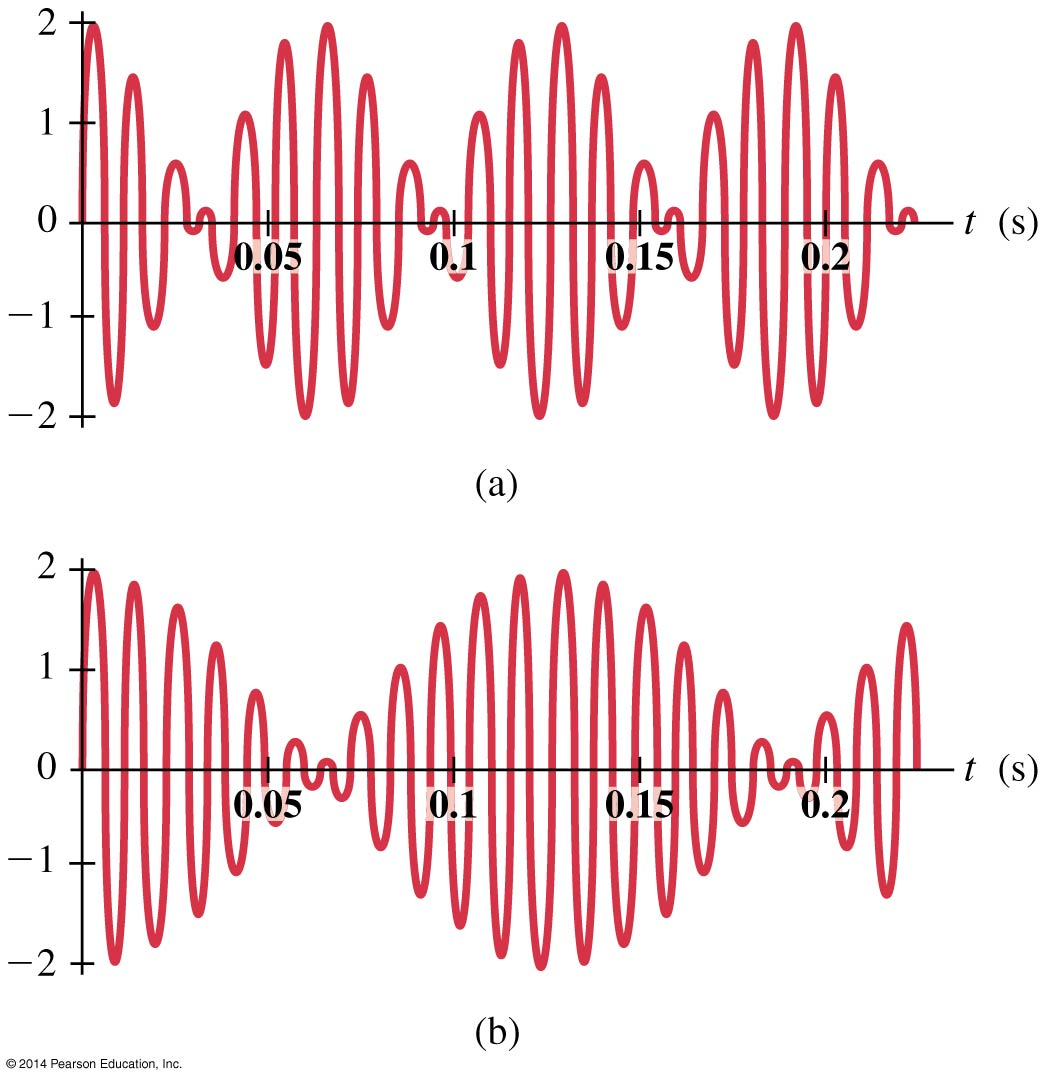
\includegraphics[width=7cm]{12_31_Figure.jpg}
    \caption{Giancolli Figure 12-31.}
    \label{12-31}
  \end{figure}
  
\end{multicols}




\myquestion (Giancoli CQ11) \answer{A}
Two waves are traveling toward each other on a rope.  When they meet the waves,
\begin{choices}
  \choice Pass through each other
  \choice Bounce off each other
  \choice Disappear
\end{choices}
\end{enumerate}



\pagebreak

\hfill

\subsection*{Selected Answers}

  \renewcommand{\enotesize}{\normalsize}
  \renewcommand{\enoteformat}{%
    \leftskip=1.8em
    \makebox[0pt][r]{\theenmark. }%
  }

  \hfill

  \begin{multicols}{2}
    \theanswers
  \end{multicols}
\hrule

\end{document}